%
%  $Description: DiFUSE - CMPS229: Storage Systems. 
%

\documentclass[10pt,twocolumn]{article}
\usepackage{times,mathptmx,fullpage}
% Allows you to put literal text into your document without having
% LaTeX try to interpret it.
\usepackage{verbatim}
% Sorts citations numerically and "combines" adjacent ones
\usepackage{cite}
% Allows you to individually label subfigures in a multi-part figure
\usepackage{subfigure}
% Allows the definition of macros that are smart about adding space
% after text in a macro
\usepackage{xspace}
\usepackage{graphicx}
\usepackage{amsmath}
\graphicspath{/}

% Redefine the percentage of the page that can be used for floats (figures,
% tables, etc.)
\renewcommand\floatpagefraction{.9}
\renewcommand\dblfloatpagefraction{.9}
\renewcommand\topfraction{.9}
\renewcommand\dbltopfraction{.9}
\renewcommand\bottomfraction{.9}
\renewcommand\textfraction{.1}
\setcounter{totalnumber}{10}
\setcounter{topnumber}{10}
\setcounter{dbltopnumber}{10}
\setcounter{bottomnumber}{10}

% Set values for float separation from text
\setlength{\floatsep}{1.5ex plus1.0ex minus 0.2ex}
\setlength{\dblfloatsep}{1.5ex plus1.0ex minus 0.2ex}
\setlength{\textfloatsep}{1.5ex plus1.0ex minus 0.2ex}
\setlength{\dbltextfloatsep}{1.5ex plus1.0ex minus 0.2ex}
\setlength{\abovecaptionskip}{0.5ex}
\setlength{\belowcaptionskip}{0.5ex}

% Don't allow widows or clubs - single lines at the start/end of a column
\widowpenalty=10000
\clubpenalty=10000

\newcommand{\latex}{\LaTeX\xspace}
\pagestyle{plain}

%------------------------------------------------------------------------- 
\begin{document}

\title{DiFUSE - A Dissident File System}

\author{
Aneesh Neelam \\
\textit{Univ. of California, Santa Cruz} \\
\textit{aneelam@ucsc.edu}
\and
Darrell D. E. Long \\
\textit{Univ. of California, Santa Cruz} \\
\textit{darrell@ucsc.edu}
}

\maketitle

\begin{abstract}

Dissidents under totalitarian governments may not have the equivalent of the United States' Fifth Amendment protections. Therefore, one cannot just encrypt their data without being subjected to rubber hose attacks. Also, traditional steganography cannot be used under such circumstances, as it will be broken eventually by the State, given enough time and effort. Even in chaotic systems, there will be a pattern of limited predictability.  We present DiFUSE, a dissident file system that combines aspects of steganography and encryption to protect data from untrusted parties, and attempts to provide the dissident with a means of plausible deniability. 

\end{abstract}

%------------------------------------------------------------------------- 
\section{Introduction}

Dissidents use many tools to protect their digital data, online identity, etc. from a totalitarian government, and each of these tools has advantages and disadvantages. Depending on the laws of the State and the legal precedents established, the dissident may be compelled to reveal incriminating data to the State \cite{gametheory}. Failure to do so can lead to severe fines and incarceration.  Therefore, it is not enough for the dissident to use the tool to conceal data or identity, but also conceal the use of such a tool from the State. 

Encryption by itself does not hide the data. If a third party analyzes the data blocks, they may not be able to make sense of them, but they can conclude that it has been encrypted. They can then ask for the key. In countries such as the United States, you cannot be legally compelled to reveal anything that incriminates you ~\cite{fifth}. However, not all States have such legal protections. Unfortunately, there are some which even torture for such information. An encrypted file system cannot be read without the decryption key(s), but such a State can compel the dissident to decrypt it or share the decryption key(s) ~\cite{gametheory,stegfs}. Steganography by itself is also not a feasible option. By analyzing the size of the data and the content, anomalies will be found and the use of steganography can be detected ~\cite{steg}. The State can eventually retrieve the dissident’s data from the disk drives. 

DiFUSE, a dissident file system, aims to provide plausible deniability for the dissident if their disk drives are ever subjected to inspection. In this paper, we shall talk about the design and implementation details of DiFUSE. Some explanations on why certain algorithms, tools, and design patterns were chosen along with their trade-offs are also described in this paper. 

In the next section, we shall see the approaches that others have taken to solve this problem of safeguarding data while maintaining plausible deniability. In Section 3 and 4, we shall describe how DiFUSE is designed and the current implementation. In Section 5, we analyze its limitations and evaluate its performance. We then discuss future work in Section 6. 

%------------------------------------------------------------------------- 
\section{Related Work}

A lot of work has been done to protect data stored on disks from third parties. Various encryption algorithms have been devised and implemented in a variety of languages and for many platforms. There are two primary kinds of encryption for data stored on disks: Full Disk Encryption and File-level Encryption. 

Full Disk encryption encrypts the entire disk, including the free space ~\cite{disksym,diskintel,diskwin}. There are ways to defeat this mechanism, however. It is possible to use a keylogger to capture the key when the user is entering it. Another method is called a cold-boot attack, where the key may be stored in RAM for comparison and since DRAM and SRAM are still readable for a few seconds after the system is shutdown, the contents of the RAM may be dumped and analyzed ~\cite{androidenc}. Various mechanisms to speed up disk encryption have been developed. Newer CPU architectures have special AES instructions and specialized hardware for AES encryption ~\cite{intelaes}. 

File-based encryption, on the other hand, encrypts files individually in the file system layer and stores them. When reading the data back, the file system seamlessly decrypts the data. IBM developed Encrypted File System (EFS) for the AIX system, which employs this method to safeguard files stored on disk ~\cite{ibmefs}. 

Both disk and filesystem level encryption suffer from the same problem: The existence of the data protected using encryption and the use of encryption mechanisms cannot be denied ~\cite{gametheory}, and they are frequently subjected to rubber hose attacks \cite{rubberhose}. 

Steganography has also been employed to safeguard data on disk. The Steganographic File System was developed to give users an element of plausible deniability that encryption alone cannot provide. Users cannot be compelled to divulge the key if the adversary is not aware that the data even exists. The user can confidently deny the existence of the data in such a case ~\cite{stegfs}. But, if data hidden using steganography can be found with some level of effort and time. This data is generally not encrypted as that can break steganography, and subsequently does not offer plausible deniability. 

An encryption tool called Truecrypt was developed that also had a plausible deniability feature. The disk is split into two volumes. One volume contains the actual data; the other contains dummy data that the user is willing to sacrifice. Two keys are used to decrypt the disk. One key only decrypts one of the volumes. Hence, the user can give away the key corresponding to the volume with dummy data, if compelled and the sensitive data in the other volume is still safe ~\cite{gametheory}. But, the disk can be carefully analyzed and the size of the volume would not add up to the size of the disk, in which case the adversary can compel the user to disclose the actual key ~\cite{truecrypt}. 

%------------------------------------------------------------------------- 
\section{Design}

DiFUSE has been implemented using the FUSE API, which is supported by many POSIX systems, including OS X, Linux, and FreeBSD ~\cite{fuse}. The dissident file system is a layer on top of the existing ``normal'' one. This is because a fully fledged custom file system or the presence of a custom kernel may be suspicious, depending on how the totalitarian government perceives the dissident. 

The dissident file system uses harmless, ``innocent'' files to ``encrypt'' sensitive files. Innocent files are those which are completely legal in the specific jurisdiction, are not suspicious for the dissident to have on his or her system and are also specific to the dissident. The sensitive file data when written, shall be XORed with an innocent file and the result is written to the underlying file system. And when reading these files via the dissident file system, the underlying file is then XORed with the corresponding innocent file to obtain the actual data. 

We know that if $\mathit{r}$ is random, then $\mathit{q = r \bigoplus d}$ is also random, regardless of what $\mathit{d}$ is. However, the ``innocent'' file cannot be made up of random data. Otherwise, it cannot be termed “innocent” anymore. Random unreadable data is also suspicious to have. 

Suppose, the sensitive data that is to be written via the dissident file system is a byte array $d$. The innocent file that must be XORed with $d$ can be $a$. Now, assuming that the innocent file is much larger than the sensitive file, the byte array $d$ will be XORed with an offset, $i$, and onward, until the size of $d$. This offset $i$ is randomly generated when writing a new file. Otherwise, it is retrieved from a store. The pseudo-random number generator must be cryptographically secure; else the offsets can be reverse engineered by analyzing DiFUSE in execution, or even compromise the security of other instances of DiFUSE on other machines if the random numbers generated are predictable. 

The file inode numbers and the respective offsets must be written to a file system store, as a file on the underlying file system itself. This file system store is also a file that understandably needs to be protected in the same manner. However, the corresponding offset for this must be determined using a deterministic method. The offset is chosen based on the cryptographic hash of a pass phrase entered when mounting the dissident file system. 

%------------------------------------------------------------------------- 
\section{Implementation}

The dissident file system is built using the FUSE API for POSIX systems. This enables compatibility across the different Unix-based and Unix-like systems. But, some aspects of the design and implementation may depend on how the POSIX interface is implemented in that operating system. Hence, we shall assume that this file system will be used on FreeBSD, Linux, and Mac OS X systems. 

For the file system to work, we need a mechanism to generate random numbers for offsets. We also need a secure hashing algorithm for calculating the offset from the passphrase for the file system store file. And we need a file system store that provides durability and consistency while being able to handle concurrent file system operations. 

\subsection{Passphrase}

The offset for the file system store is calculated using SHA-512, one of the algorithms in the SHA-2 family of cryptographic hashing algorithms. Running SHA-256 on the passphrase results in a 64-byte hash. Taking the most significant byte as the offset, we can then read the store file. 

\subsection{Random Number Generator}

For generating cryptographically secure random numbers, only hardware-based or at least hardware-backed random number generators must be used. Assuming the dissident will not be able to carry specialized hardware random number generators, we can only rely on hardware-backed ones. 

We use the ``/dev/random'' device file, which uses environmental noise for its entropy pool to obtain the random seeds for the pseudo-random number generator. Implementations of /dev/random by all three systems, are designed to be cryptographically secure and even long lasting keys like SSH, GPG and SSL keys are generated from such hardware-backed entropy systems. 

We can assume that the dissident file system shall be used on a system which has user interaction, and not a server which does not have these sources of entropy. However, some servers also require cryptographically secure random numbers for securing data on the network. Hence, such servers are configured to obtain entropy for random number generation from other sources on the internet. 

/dev/random Implementations: 
\begin{itemize}
\item On Linux systems, the /dev/random device takes environmental noise from device drivers into an entropy pool. From this pool cryptographically secure random numbers can be generated.  On Linux, however, /dev/urandom does not block if a sufficient entropy pool is not present. Hence, /dev/urandom on Linux is not recommended for cryptographic algorithms \cite{linuxrandom}. 
\item On Mac OS X, the /dev/random device uses the Yarrow algorithm devised by John Kelsey, Bruce Schneier, and Niels Ferguson, and implemented by Apple. It uses various sources of entropy to seed its random number generator \cite{yarrow}. 
\item On FreeBSD, the /dev/random device uses the Fortuna pseudo random number generator devised by Niels Ferguson and Bruce Schneier, and implemented by the FreeBSD developers. It also uses various sources of entropy to seed its random number generator and is similar to Yarrow \cite{fortuna}. 
\end{itemize}

\subsection{File System Store}

BerkeleyDB is an embedded key-value database library that can be incorporated into applications \cite{berkeleydb}. It supports concurrent requests, which are necessary for a file system. It is supported on FreeBSD, Linux, and Mac OS X. 

Since the inode numbers do not change unless the file is moved, it can be used as a key for the file system store \cite{astmos}. The offsets must be stored with the respective inode numbers in the dissident file system store. For a randomly generated offset $i$, and a file size $s$, the corresponding innocent file needed ranges from $i$ to $i + s$. If $i + s$ becomes greater than the size of the innocent file itself, the modulus operator can be used to go back to the start of the file. This provides an apparent endless continuity to the innocent file. 

When appending or updating data in-place to an existing file, one must calculate the starting offset by taking the existing offset and adding the specified offset or the original file size to obtain the offset of the innocent file. 

%------------------------------------------------------------------------- 
\section{Evaluation}

We evaluate the performance, and also analyze the possible threats and attack vectors for the current implementation. We also some describe some of the trade-offs in the design. 

\subsection{Threats and Trade offs}

The adversary is assumed to be a government which is highly motivated and capable with almost unlimited resources. To reverse engineer the offsets, one must be able to break the randomness of the machine, and the SHA-512 algorithm. Since these algorithms are known to be cryptographically secure for now as breaking them is computationally unfeasible for the foreseeable future. Therefore, we can use them to generate random numbers for offsets and to hash the passphrase. Brute-forcing the offsets can also be attempted. However, the feasibility of this task depends on the size of the innocent file and the number of sensitive files. 

It is possible to break the randomness of the machine by compromising the entropy sources of the random number generators. However, that only compromises the random numbers generated since then, not the ones already generated before. 

Deliberate manipulation of the sensitive files or even the innocent files from the underlying normal file system can destroy the data. The underlying file system does not do so as part of its normal execution, the user themselves or a program must deliberately be instructed to manipulate the data from the underlying file system for the sensitive files to be destroyed. The file names (and paths) are still unique in this case, and hence, the underlying normal file system would not overwrite these files unless explicitly performed. 

We are not XORing random data at all; we are only choosing non-random innocent data at random. This is a tradeoff as it may be more statistically insecure than using actual random data. However, we assume that innocent files are easier to pass off than random files. Also, if the innocent files themselves are compressed files, the entropy of the innocent file itself is higher, making the innocent data itself more ``random-like'' \cite{compression}. 

There are still XORed files all over the file system; these represent the actual sensitive data. However, since these files are generally smaller in number and smaller in size when compared to the ``innocent'' files used, the dissident may be able to pass them off as file system corruption. However, we understand that this is a major concern as rubber hose attacks become possible \cite{rubberhose} and as part of future work, this can be addressed. 

\subsection{Performance}

DiFUSE's performance was evaluated and compared to the native file system present. All tests were performed on commodity hardware, in this case, a 15" Macbook Pro (mid-2015). The native file system is the default HFS+, and Mac OS X's FileVault disk encryption is enabled. 

Since XORing data from multiple different sources requires more computation than only reading one source to read a file, it is expected to be slower than the native file system. However, since that is not the goal this overhead can be termed acceptable. 

The following tools were used for benchmarking: 
\begin{itemize}
\item dd \& sync
\item bonnie++
\end{itemize}

The read performance of DiFUSE is slightly above the native file system. We believe this anomaly occurs because the read operation is performed on the same file every time, and hence the same chunk of the innocent file is taken and XORed with the sensitive file. This chunk can be cached in memory by the operating system, thereby improving performance. 
\begin{figure}[thpb]
  \centering
  	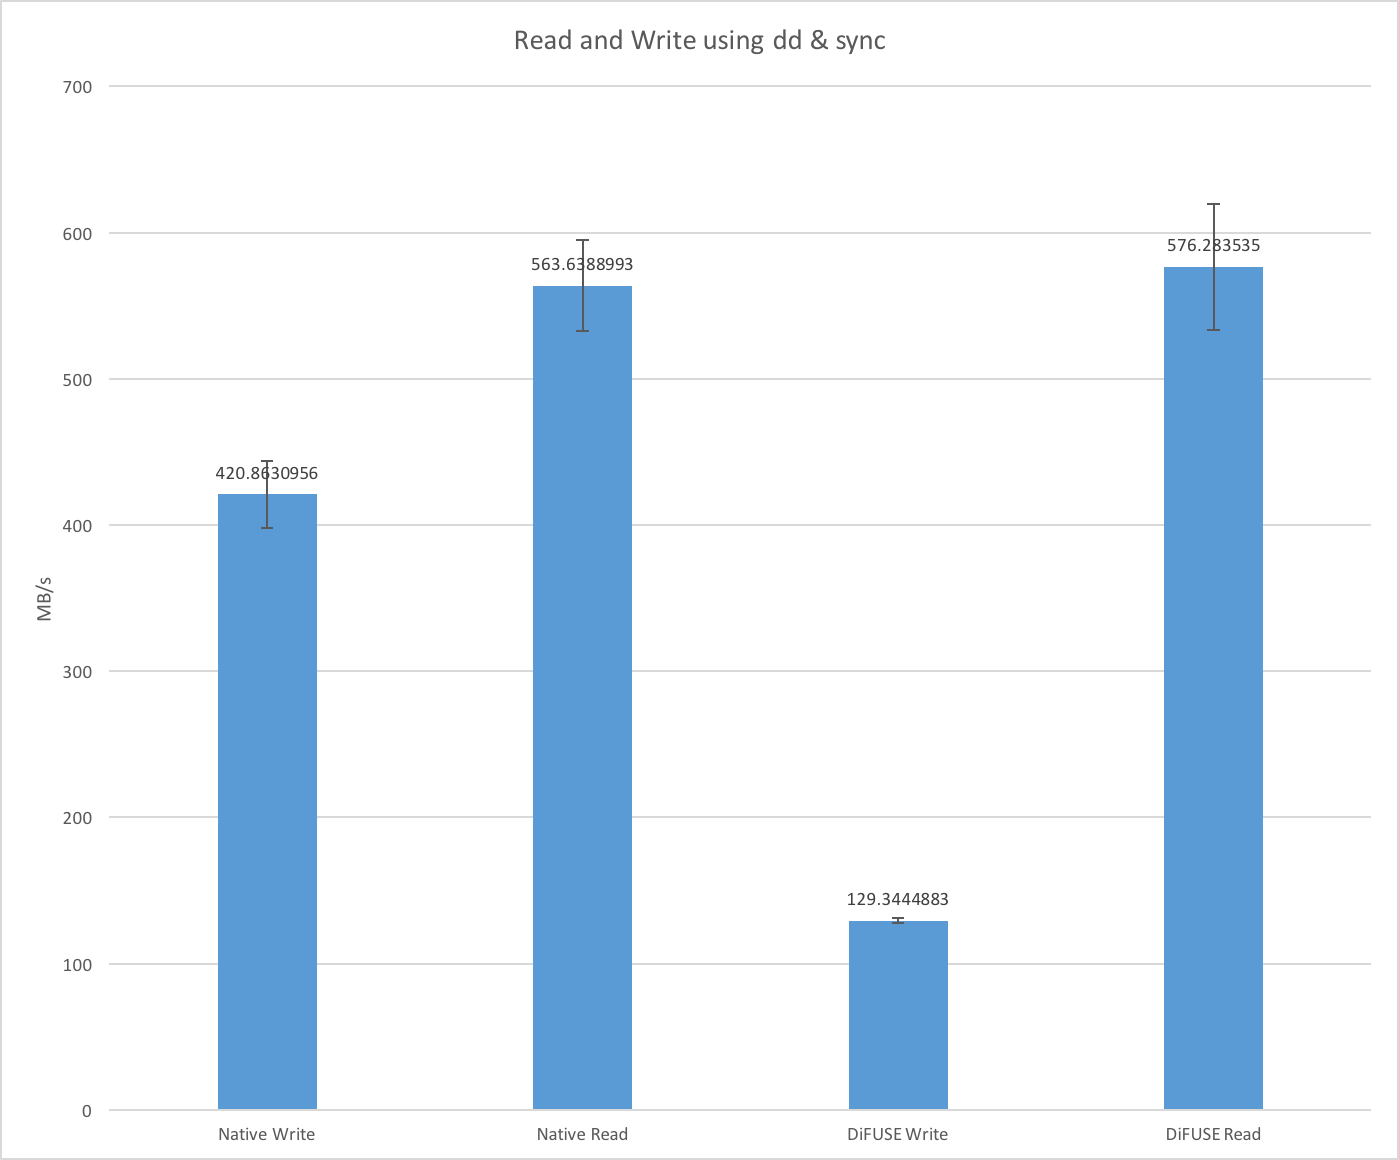
\includegraphics[width=\columnwidth]{dd}
    \caption{18 runs of dd \& sync of 1000 blocks of 100k size each. }
	\label{fig:dd}
\end{figure}

The Bonnie++ 1.9.7 benchmark test large file IO and also the creation and deletion of small files \cite{bonnie}. Bonnie++ on DIFUSE has been used for the following benchmark. 
\begin{figure}[thpb]
  \centering
  	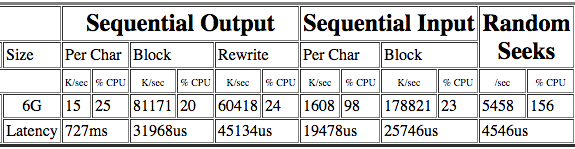
\includegraphics[width=\columnwidth]{bonnie1}
    \caption{Bonnie++ on DiFUSE - 6 GB large file: CPU usage, Throughput and Latency}
	\label{fig:bonnie1}
\end{figure}

\begin{figure}[thpb]
  \centering
  	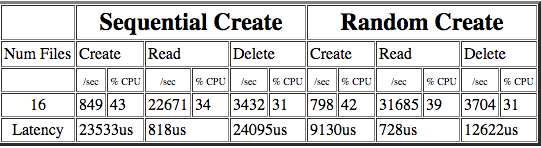
\includegraphics[width=\columnwidth]{bonnie2}
    \caption{Bonnie++ on DiFUSE - 16 small files: Throughput and Latency}
	\label{fig:bonnie2}
\end{figure}

%------------------------------------------------------------------------- 
\section{Future Work}

Since, the presence of sensitive XORed data as normally unreadable files on the native file system is suspicious, a new method to store this data on the disk must be devised. 

One such method could be storing in the free blocks of the underlying file system. Free space on a file system normally contains previously deleted data. When a disk is wiped using a secure method of erasing data, these free blocks are indistinguishable from random data. Hence, the sensitive files could be stored here. However, the native file system may overwrite this data as it considers it free space. Therefore, redundancy and error correcting mechanisms could be used for this sensitive data. Redundancy and error correcting codes enable the dissident file system to reconstruct the sensitive data blocks if the data is ever overwritten. 

Another method could be to mark the blocks where the sensitive data is stored as bad blocks \cite{badblocks}. Bad blocks are considered to be permanently damaged, and the native file system avoids them when writing to disk. Hence, ``fake'' bad blocks could be marked, and sensitive data could be stored on them. Actual bad blocks on the disk can be avoided normally. 

However, both approaches may require access to the underlying file system's data structures from the dissident file system. We are looking to see if that is technically feasible without modifying the underlying file system, and also if it can be done in a file system agnostic manner. 

%------------------------------------------------------------------------- 
\section{Conclusion}

DiFUSE is a work in progress towards a true dissident file system, where sensitive information could be stored on the disk, encrypted and also hidden from any external parties. A file system for dissidents allows them to resist totalitarian regimes with greater data security and physical safety from rubber hose attacks. 

%------------------------------------------------------------------------- 
\bibliographystyle{latex8}
\bibliography{latex8}

\end{document}
